\documentclass[12pt, a4paper]{article}
\usepackage[spanish]{babel}
%\usepackage{a4wide}
\usepackage{amsmath}
\usepackage{amssymb}
\usepackage{amsthm}
\usepackage{color}
\usepackage{hyperref}
\usepackage{makeidx}
\usepackage{float}
\usepackage[margin=1.0in]{geometry}
\usepackage{caratula}
\usepackage{pdfpages}

\usepackage{listings}\usepackage{color}
\usepackage{textcomp}\definecolor{listinggray}{gray}{0.9}

\definecolor{lbcolor}{rgb}{0.9,0.9,0.9}
\usepackage{a4wide}

\lstset{
      language=C++,
      basicstyle=\small\sffamily,
      columns=fullflexible,
      upquote=true,
      extendedchars=true,
      texcl=true,
      mathescape=true,
      showspaces=false
                }



\makeindex

\begin{document}

\index{Caratula}
%Estos son los parametros para la caratula
\materia{WHPC13}
\submateria{Trabajo final}
\titulo{T\'ecnicas de paralelismo y HPC}
\fecha{26 de Julio de 2013}
\integrante{Ferreria, Manuel}{}{m.ferreria@gmail.com}
\resumen{Estudio de t\'ecnicas de paralelismo con varias herramientas y tenicas en CPU y GPU
}

\maketitle

\pagebreak

\tableofcontents

\pagebreak
\index{Ejercicio1}
\section{Ejercicio 1}

\subsection{Introducci\'on}
El ejercio 1 consiste en realizar un producto vectorial sencillo, empleando distintos m\'etodos.
Se utiliz\'o la libreria thrust para las versiones en C++ de CPU y de GPU, y se uso PyCUDA para
la version en Python.

La soluci\'on para la libreria thrust es utilizar la funci\'on transform, que toma varios parametros
de entrada, donde se definen los operandos, el lugar de destino y el operador. En nuestro caso,
se aplic\'a transform de la siguiente manera:

\small{\texttt{
    thrust::transform(D1.begin(), D1.end(), D2.begin(), D3.begin(),\\
                       thrust::multiplies<float>());
               }}

Esto se define como: Tomar los datos de D1, de comienzo a fin, combinarlo con el dato de D2 al aplicarle la funci\'on 
de \texttt{thrust::multiplies<float>()} y dejarlo en D3. Una ventaja de thrust es que es totalmente 
portable entre CPU y GPU. Otra ventaja es que es muy idiomatico de C++, no hay ninguna construcci\'on muy rara
que no se encastre en el lenguaje. 


\subsection{Resultados}
\def \hrwidth {300pt}


  \begin{figure}[H]
 \begin {center}
 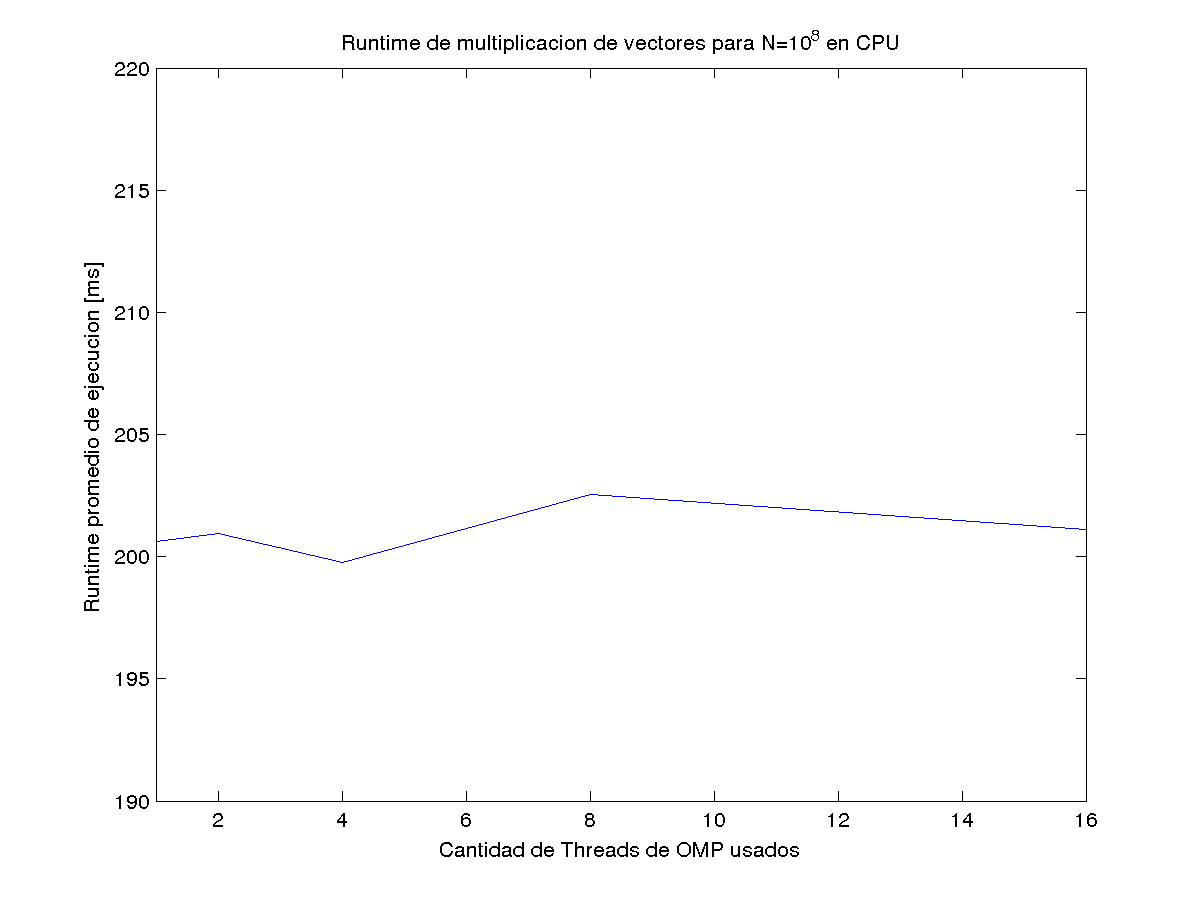
\includegraphics[width=\hrwidth]{plots/ej1omp.png}
 \end {center}
 \caption{Runtime del ej1 en Thrust con OMP, en funcion de la cantidad de threads, para una longitud de vectores $N=10^8$}
 \label{fig:ej1OMP}
 \end{figure}

 \begin{table}[H]
    \begin{tabular}{l| r}
        \textbf{M\'etodo} & \textbf{ Runtime [ms] }\\ \hline
    1 OMP Thread         & 200.598      \\
    2 OMP Thread          & 200.963      \\
    4 OMP Thread          & 199.766      \\
    8 OMP Thread  & 202.534      \\
    16 OMP Thread & 201.127      \\
        CUDA M2090 & 11.035 
    \end{tabular}
\end{table}



 Como se puede ver en el gr\'afico y la tabla de la figura \ref{fig:ej1OMP}, casi no varian los runtimes a pesar de tener
 muchos threads. Esto se debe a que el costo de generar y spawnear threads nuevos es tan alto que el procesador
 deberia hacer m\'as c\'alculo por core en vez de paralelizar m\'as el problema. Esto es un claro ejemplo
 de una tarea que es demasiado chica para threadear, e incluso con un problema relativamente grande de $10^8$ 
 elementos, no vale la pena paralelizarlo con CPU.

 Comparado contra la placa Nvidia con CUDA, podemos apreciar la diferencia de velocidad notablemente. Esto igual no toma
 en cuenta el tiempo de transferencia de memoria, por lo cual puede llegar a ser enga\~noso a veces el tiempo de runtime
 en las comparaciones CPU/GPU.


\pagebreak


\index{Ejercicio2}
%\section{Ejercicio 2}

El ejercio 2 consiste en realizar con CUFFT y FFFTW una FFT de real a complejos y la inversa,
y comprobar que ambas son inversas entre si (es decir, devuelven los valores originales).
Se utilizaron la libreria Thrust y CUFFT para las versiones en C++ de CPU y de GPU.

El ejercicio planteando incluia una funcion $f$ que es aplicada a un arreglo en la memoria de la GPU que contiene
una secuencia de $N$ numeros, fijado $N=1048576=2^{20}$. Este numero es bueno porque al ser m\'ultiplo de 2,
CUFFT reserva una cantidad exacta de m\'emoria, y no tiene que paddear ni redondear, ayudando a la performance 
\'optima de las funciones.

El c\'odigo ya escrito en el enunciado realizaba una FFT de real a complejos a un arreglo del 0 a N al que se
le aplicaba una funci\'on $f$. La tarea que realizamos nosotros fue la de obtener la inversa de este valor.
Para eso, aplicamos las funciones definidas en la API de CUFFT, pero que deshagan las transformaciones.

Es decir, si la ida fue armada como 
\begin{itemize}
    \item Armar plan R2C para N elementos
    \item Disponer de un vector en la placa/en memoria para N/2+1 elementos para guardar resultado
    \item Correr el plan R2C con CUFFT/FFTW
\end{itemize}

La vuelta se va a armar como

\begin{itemize}
    \item Armar plan C2R para N elementos
    \item Disponer de un vector en la placa/en memoria para N elementos para guardar resultado
    \item Correr el plan C2R con CUFFT/FFTW
\end{itemize}


El detalle m\\as importante de esto fue darnos cuenta como recuperar los valores originales. Parece que es trivial
ya que vamos y volvemos con las ejecuciones de los planes, pero hay un comentario corto que esta en el manual de CUDA y de 
FFTW. Este dice que FFTW / CUFFT no normalizan, por lo que eso lo tiene que hacer uno. Es decir, cuando imprimimos
los valores originales para comprobar la exactitud de la ida y vuelta de la FFT, tenemos que reescalar el valor
final haciendo una division por la cantidad de elementos en el arreglo. Cuando nos percatamos de eso, fue trivial
la comparacion entre el dato de input y el de output.

  \begin{figure}[H]
 \begin {center}
 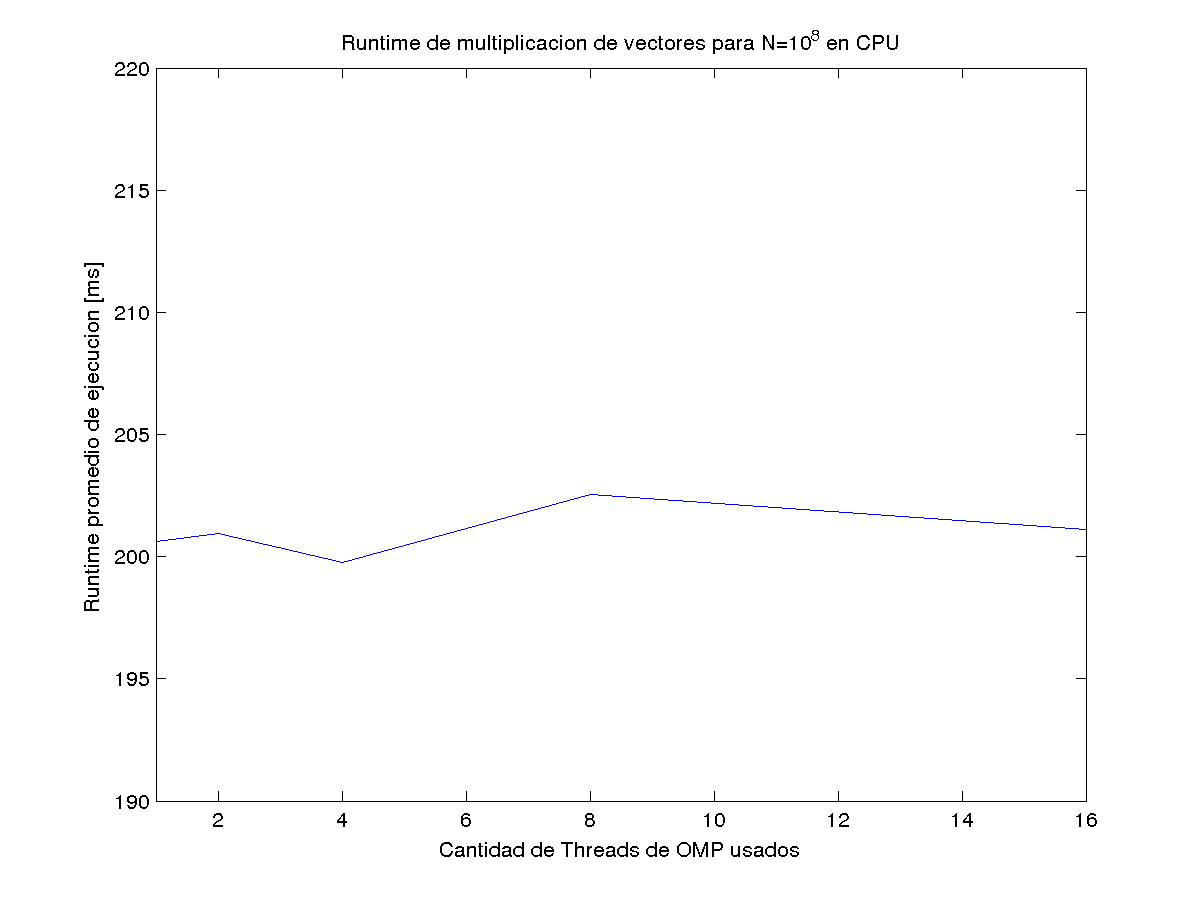
\includegraphics[width=\hrwidth]{plots/ej1omp.png}
 \end {center}
 \caption{Runtime del ej1 en Thrust con OMP, en funcion de la cantidad de threads, para una longitud de vectores $L=10^8$}
 \label{fig:ej1OMP}
 \end{figure}

\begin{table}
    \begin{tabular}{l|l}
        \textbf{M\'etodo} & \textbf{ Runtime [ms] }\\ \hline
    1 OMP Thread         & 200.598      \\
    2 OMP Thread          & 200.963      \\
    4 OMP Thread          & 199.766      \\
    8 OMP Thread  & 202.534      \\
    16 OMP Thread & 201.127      \\
        CUDA M2090 & 11.035 
    \end{tabular}
\end{table}



 Como se puede ver en el gr\'afico y la tabla de la figura \ref{fig:ej1OMP}, casi no varian los runtimes a pesar de tener
 muchos threads. Esto se debe a que el costo de generar y spawnear threads nuevos es tan alto que el procesador
 deberia hacer m\'as c\'alculo por core en vez de paralelizar m\'as el problema. Esto es un claro ejemplo
 de una tarea que es demasiado chica para threadear, e incluso con un problema relativamente grande de $10^8$ 
 elementos, no vale la pena paralelizarlo con CPU.

 Comparado contra la placa Nvidia con CUDA, podemos apreciar la diferencia de velocidad notablemente. Esto igual no toma
 en cuenta el tiempo de transferencia de memoria, por lo cual puede llegar a ser engañoso a veces el tiempo de runtime
 en las comparaciones CPU/GPU.


\pagebreak


\index{Ejercicio3}
%\section{Ejercicio 3}

\subsection{Descripci\'on}
El ejercio 3 consiste en completar una fracci\'on de la simulaci\'on de los avances de los frentes magn\'eticos
en interfaces de medios desordenados. Para eso se gener\'o un modelo basado en mec\'anica cl\'asica, usando
\textit{splines} para trazar las curvas de las particulas y \textit{springs} para delimitar el frente.

El c\'odigo fue hecho usando la librer\'ia \texttt{Thrust} para poderlo correr en CPU y GPU indistintamente.
Tambien se utiliz\'o un random number generator especial, basado en contadores, para no tener que almacenar las posiciones 
hist\'oricas de cada particula. Esto hace manejable los tama\~nos de de mem\'oria de modo que entren en las placas
aceleradoras GPGPU. 

\subsection{TODOs}
El primer \texttt{TODO} era relacionado al RNG. Este TODO se\~nalaba que habia un error con respecto al
uso del RNG en el caso del ruido t\'ermico. Habia que entender como funcionaba un counter-based RNG para
poder entender cual era el error ahi. El problema radicaba en como obtener n\'umeros aleatorios no correlacionados
pero que sigan siendo reproducibles de la misma manera que los usados para el desorden del medio. 
Los counter-based RNG toman dos parametros, un counter y una key, y devuelven un numero aleatorio. Llamar
con los mismos parametros al RNG siempre devuelve el mismo n\'umero. Esto indica que para obtener 
el siguiente valor de la secuencia random, habr\'ia que modificar el counter. Sin embargo, quisieramos
obtener valores aleatorios tambien para el otro ruido, y debieramos seedearlos distinto para que no
haya ninguna correlaci\'on entre ellos. Para eso, habria que variar la key, y setearla al seed correspondiente.

Los CBRNG usados aca toman como key el valor del thread donde estan haciendo el computo, y como counter 
la uni\'on de un seed de cada fuente de numeros aleatorios con el $u$ usado, donde $u$ es la posici\'on del mon\'omero
actual. De esta manera los valores random son reproducibles hacia atras y hacia adelante.

Dicho todo esto, el FIXME consistia en entender la teoria de los CBRNG y ver que el uso que se le estaba dando
no generaba valores aleatorios diferentes, sino que los podia repetir. La soluci\'on consistia en hacer que el ruido
t\'ermico dependiera del tiempo de la simulaci\'on, es decir, que no pueda volver para atras el ruido termino.
Esto se hacia duplicando el mecanismo usado anteriormente y cambiando el seed al seed2 y el $u$ por el $t$ de la simulaci\'on.


El segundo \texttt{TODO} se referia al c\'alculo de dos propiedades de la interfaz, la velocidad y la posicion del centro de masas.
Recordemos que la velocidad se calcula como $V = \frac{\Delta x}{\Delta t}$ y el centro de masas (dadas las hipotesis del problema)
se calcula como $P = \frac{\Sigma_i P_i}{L}$. Para calcular el centro de masas, debemos obtener la posicion de cada uno de los
puntos y promediarla. Como el problema son $L$ puntos equiespaciados en la coordenada $y$, tomamos solamente los valores 
de X para obtener el centro de masas. Esto se traduce en un c\'odigo de thrust de reduce asi: \\
\texttt{ REAL center\_of\_mass = reduce(u\_it0, u\_it1, 0.0) / L;}\\
Esto hace una suma de todos las posiciones en X de las particulas y las promedia al dividirlas por L (fuera de la placa).

Para obtener la velocidad del centro de masas, deberiamos ver cuanto cambio su posici\'on con respecto del tiempo, $\Delta t$.
Para eso, antes de la iteraci\'on de euler inmediata anterior al calculo de propiedades, nos guardamos todas las posiciones
de las particulas (podria reducirse el uso de memoria haciendo un reduce ahi mismo).
Luego el c\'odigo relevante es:\\
\newcommand*\justify{%
  \fontdimen2\font=0.4em% interword space
  \fontdimen3\font=0.2em% interword stretch
  \fontdimen4\font=0.1em% interword shrink
  \fontdimen7\font=0.1em% extra space
  \hyphenchar\font=`\-% allowing hyphenation
}
\texttt{\justify{REAL velocity =  (( (L*center\_of\_mass) - reduce(u\_old.begin()+1,u\_old.end()-1,0.0) 
                                 ) / L  
                                 ) /Dt;  
                             }}\\
Con esto obtenemos el delta posicion arriba, y primero lo dividimos por la cantidad de elementos para obtener el promedio de los
delta por punto, y luego lo dividimos otra vez por el delta tiempo para obtener la tasa de variacion de la posicion en funcion
de un step de tiempo, es decir, la derivada de la posici\'on en funci\'on del tiempo, que es la velocidad del centro de masas.


 \begin{figure}[H]
 \begin {center}
 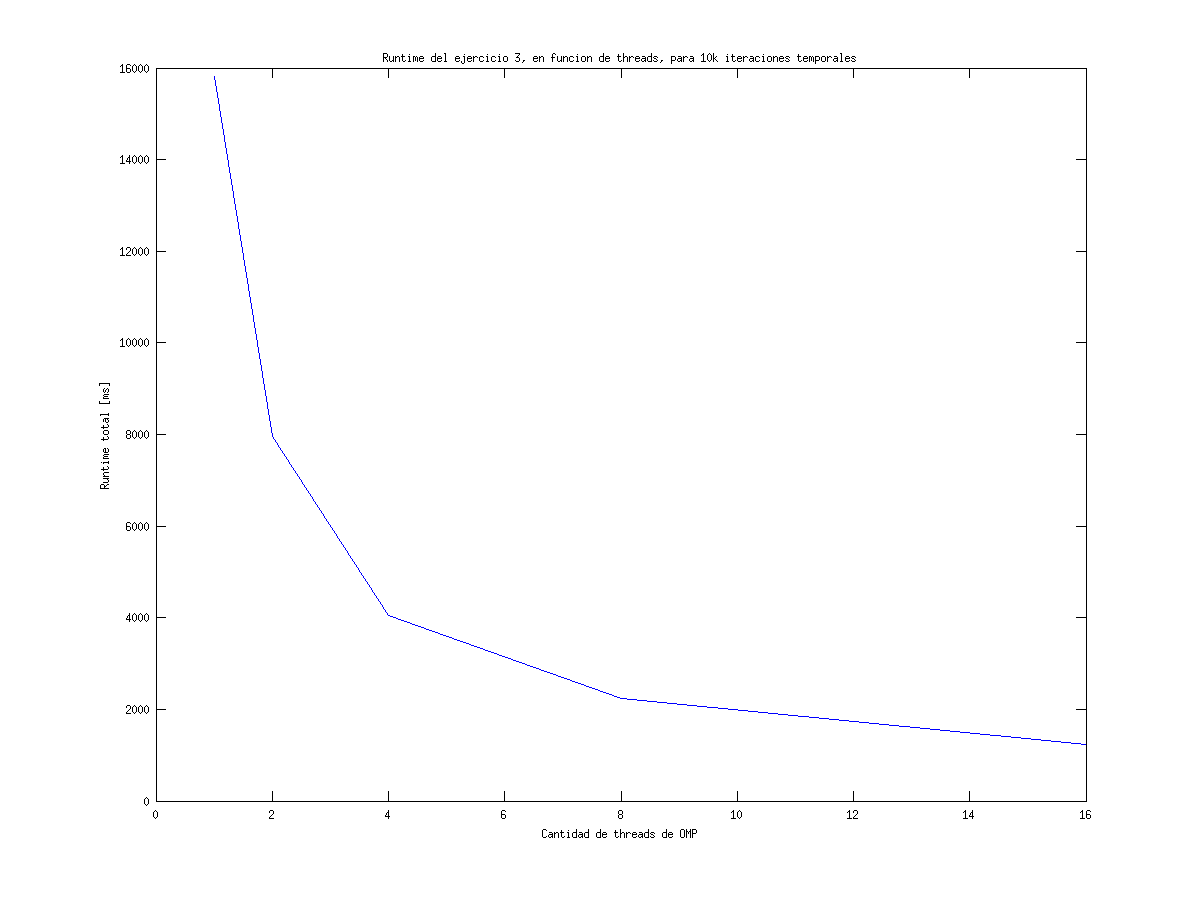
\includegraphics[width=\hrwidth]{plots/ej3omp.png}
 \end {center}
 \caption{Runtime del ej3 en Thrust con OMP, en funcion de la cantidad de threads, para 10k iteraciones temporales}
 \label{fig:ej3OMP}
 \end{figure}

 \begin{table} [H]
    \begin{tabular}{l|r|r|r}
        \textbf{M\'etodo} & \textbf{ Runtime Total [ms]}& \textbf{Tiempo fuerzas [ms]} & \textbf{Tiempo euler [ms]}\\ \hline
        1 OMP Thread         & 15861.80      & 15240.20  & 577.91\\
   2 OMP Thread          & 7971.23     & 7654.43 &309.73  \\
   4 OMP Thread          & 4072.82     & 3888.24 & 162.07 \\
   8 OMP Thread  & 2235.89     & 2130.46 & 111.05 \\
   16 OMP Thread & 1249.57     & 1132.09 & 93.87 \\
       CUDA M2090 & 473.18  & 290.505 & 176.06
   \end{tabular}
   
\end{table}


En el gr\'afico de la figura \ref{fig:ej3OMP} junto a la tabla correspondiente, podemos apreciar que este problema escala
increiblemente bien. En efecto, como el c\'alculo de casi todo es independiente, y solo se comparten pocos datos en un momento,
el problema puede escalar casi linealmente. La placa nVidia, sin embargo, sigue siendo un orden de magnitud m\'as rapida que
lo m\'aximo que podemos alcanzar usando un solo procesador Xeon en el servidor.
Comparando en la tabla con la placa GPGPU, extrapolando, podriamos concluir que equivale a un procesador de mas de 32 threads. 
Seria interesante probar este experimento en una Xeon Phi, a ver si realmente se puede comparar la performance de ambos dispositivos,
como dicen los fabricantes.

Un detalle interesante surge de ver la discrepancia en porcentaje de tiempo invertidos en las distintas cuentas. Ac\'a se puede apreciar
la potencia pura de la placa; el fragmento de codigo de fuerzas se acelera muchi\'simo. Esto se puede aplicar tanto por el hecho de
que se realizan las cuentas totalmente paralelas en distintos threads y que ademas se aprovecha el fuerte de la placa que son
las instrucciones sin condicionales. De haber algun if en ese codigo, por minusculo que sea, los valores de runtime serian bastante
mas desfavorables. Sin embargo, en el c\'alculo de paso de euler, es mucho peor la performance comparado contra incluso 4 threads OMP.
Es de creer que esto puede ser porque en si son bastantes pocas cuentas; $2^{16}$ elementos son relativamente pocos para tener 
tan baja intensidad aritm\'etica. Esto hace que se preste mejor la opcion vectorizada de calculos comparado contra la opcio\'n 
many threads de CUDA. 


\pagebreak


\end{document}
